\documentclass[12pt]{article}
\usepackage[utf8]{inputenc}
\usepackage{style}
\usepackage{graphicx}
\usepackage{setspace}
\usepackage{url}

\title{418 Final Report}
\author{changhem, jjbrenna}
\date{April 2022}

\begin{document}

\maketitle

\doublespacing % Double spaced document

\section{Summary}

Our goal is to investigate ways of parallelizing the computation in the inference of the Long Short-Term Memory (LSTM) neural network architecture. %  in order to achieve computational speedup
We designed a parallelism scheme that exploits how the computation in different layers of an LSTM can be executed concurrently.
We came up with multiple implementations and study their performance characteristics on CPU.
Our best performing implementation achieves a 36x speedup on 64 cores, with the possibility of an even higher speedup with problem scaling.
We also compared our layer-wise parallelism to the more commonly used parallelism over matrix operations and found that dedicating cores to layer-wise parallelism is more efficient.
Finally, we compare our method to a GPU implementation and found that, due to the embarrassingly parallel nature of the matrix operations, using the GPU gives better performance at higher batch sizes.

\section{Background}

% LSTM cell figure
\begin{figure}
    \centering
    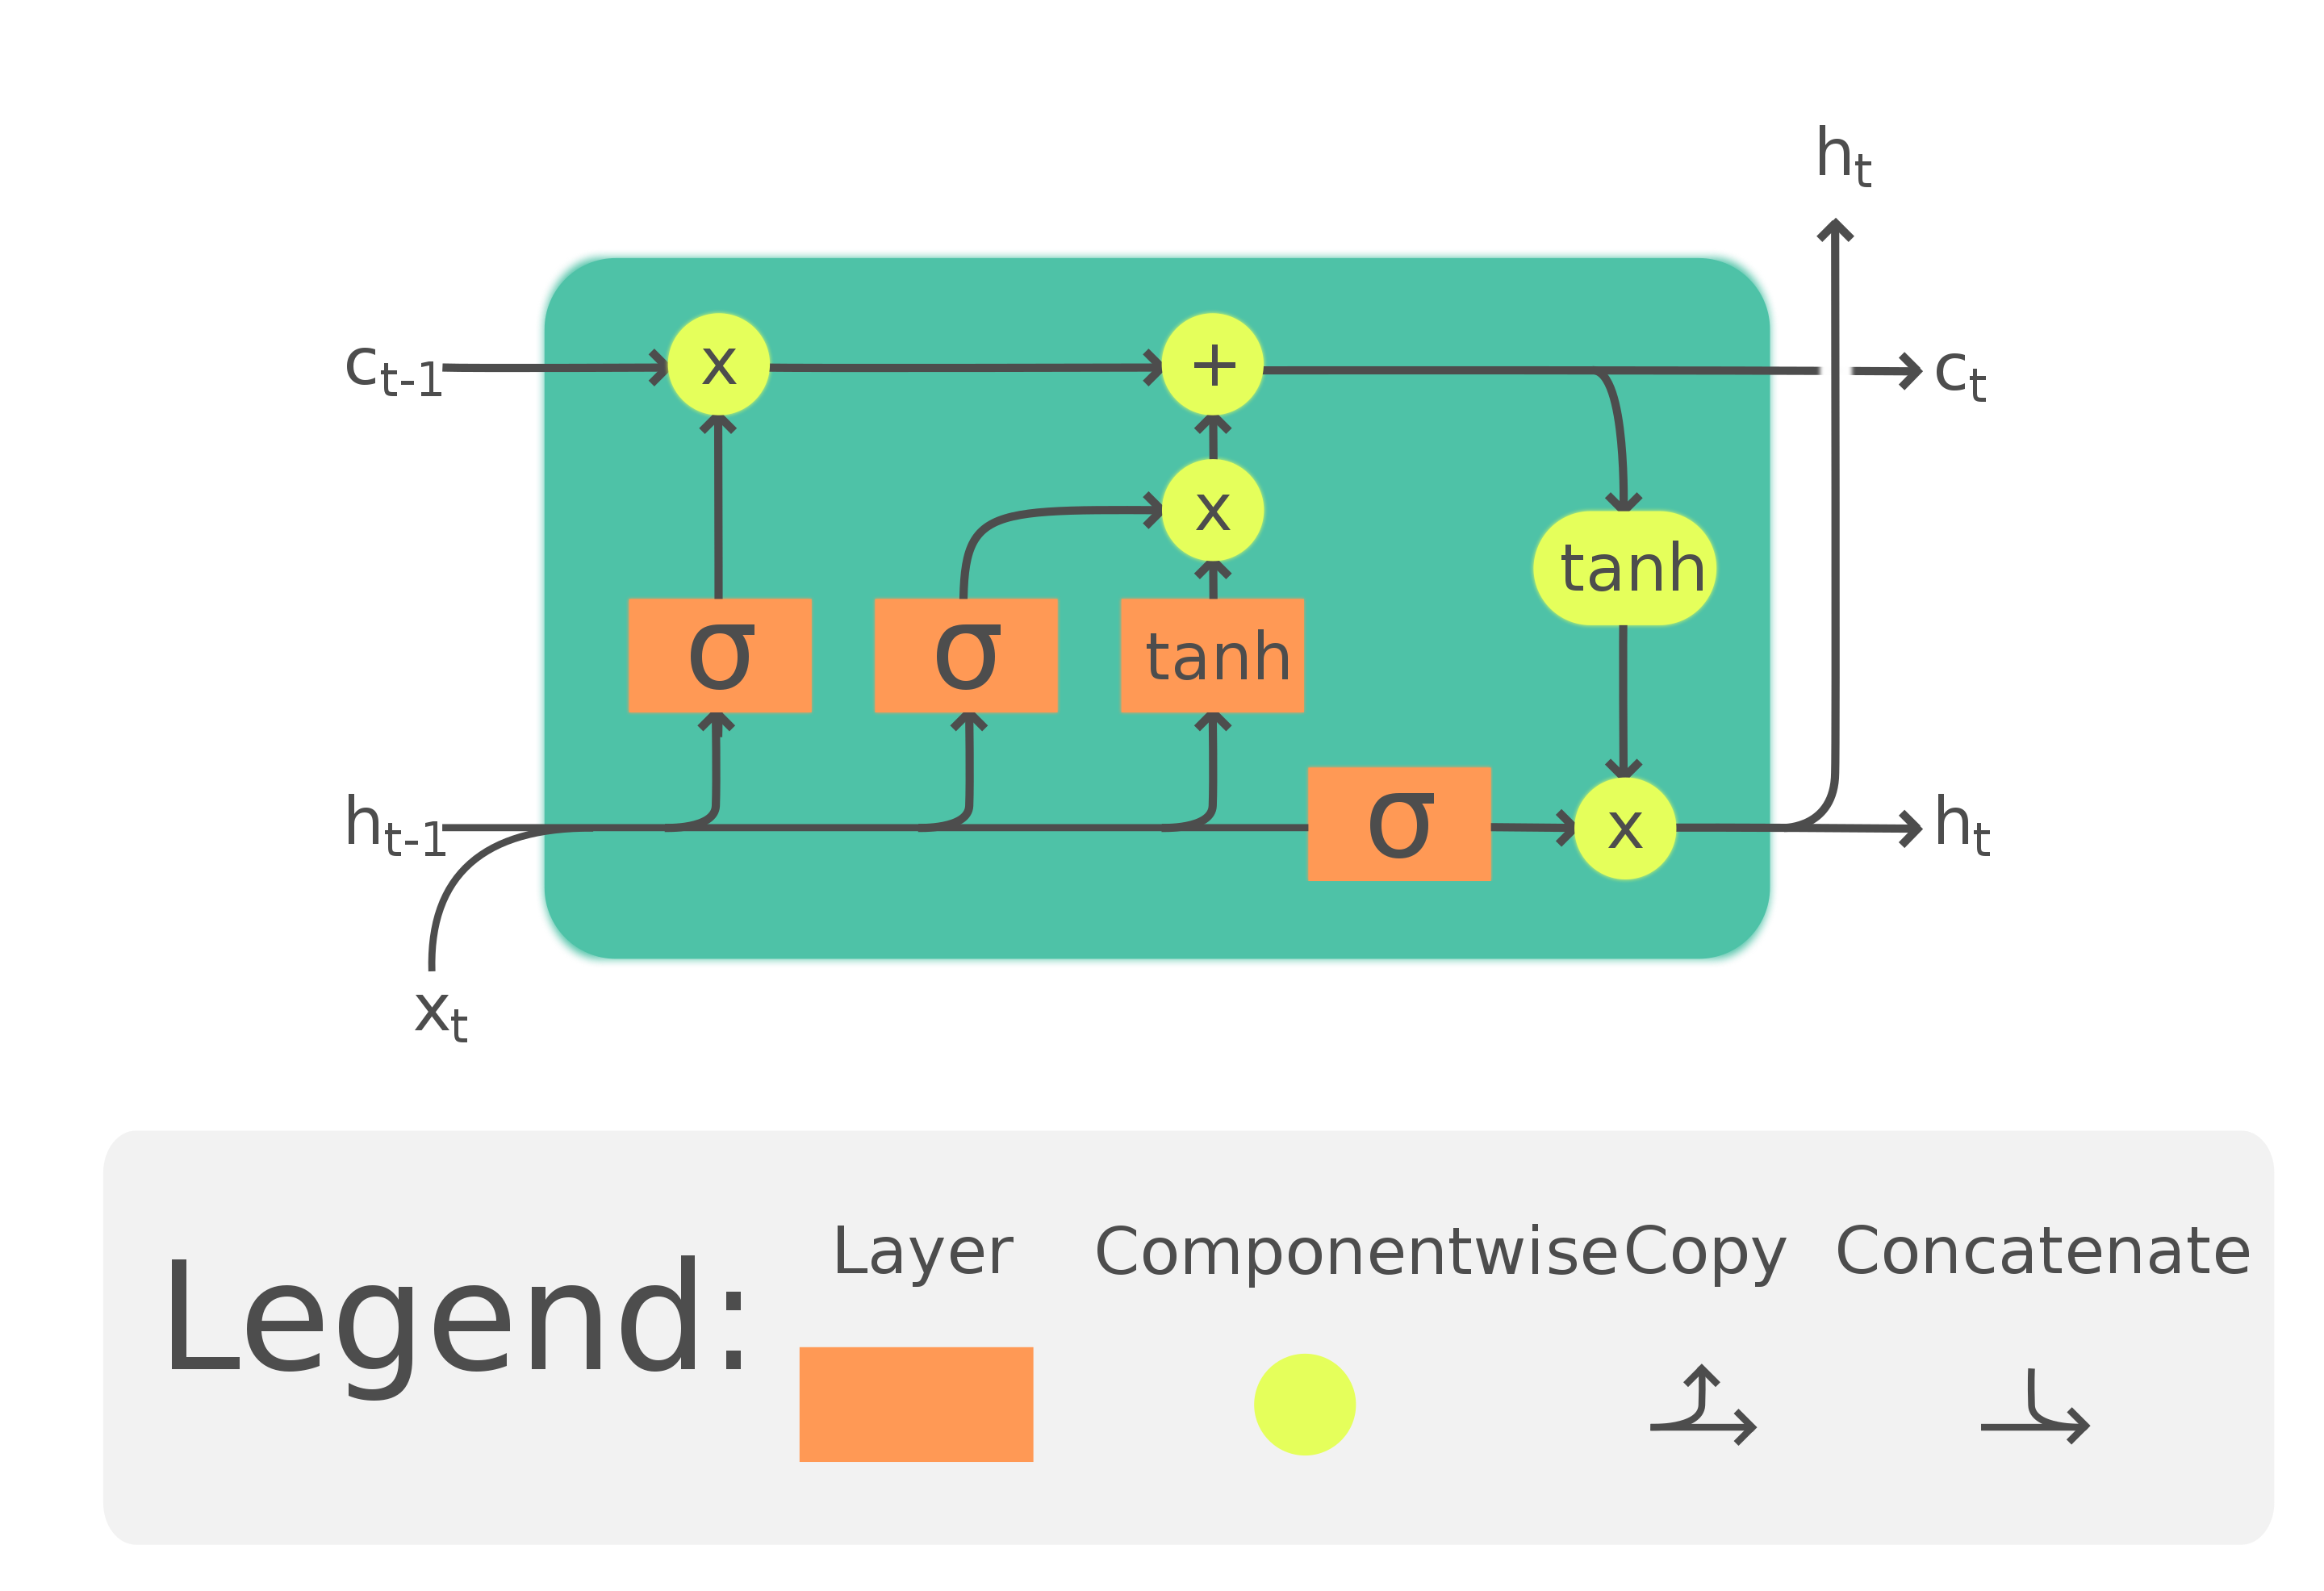
\includegraphics[width=12cm]{LSTM_Cell.png}
    \caption{Computation done in an LSTM cell~\cite{wiki:lstm}}
    \label{fig:lstm_cell}
\end{figure}

% General LSTM description
LSTM is a neural network model used to handle sequences of input. Its cells' stateful nature means that it can remember information throughout the processing of a data sequence. This makes it especially good at processing data with a sequential order, such as texts, video and audio.

% Describe the computations done by an LSTM cell
An LSTM cell has a hidden state and a memory state, which allows it to keep track of the information from previous time steps.
In order to update its hidden/memory states, the LSTM cell takes in an input and performs some computation on it, which is the expensive portion of LSTM inference.
The main computation in an LSTM cell are mathematical operations, such as element-wise arithmetic operations on matrices (e.g. addition, multiplication, sigmoid, tanh) and matrix multiplication (Figure~\ref{fig:lstm_cell}).

% Talk about dependencies in LSTM
An LSTM is typically composed of many layers of cells.
The output of one layer is used as the input to the next layer, which creates a dependency across layers.
Because LSTM cells are assumed to process elements in sequential order, there is also a dependency across time steps.
The dependency graph is illustrated in Figure~\ref{fig:wavefront_parallelism}.

% What can be parallelized?
Currently, LSTM inference mainly exploits parallelism that exists in the matrix operations. In this project, we propose a different parallelization scheme.
Because of the layered structure of an LSTM, different layers can be updated in parallel as long as dependencies are satisfied. This provides an opportunity for what we'll call layer-wise parallelism.
We will explore whether it is more beneficial to pursue mathematical parallelism, layer-wise parallelism or a combination of the two when resources are limited.

% TODO: speedup up to depth


\section{Approach}

% Wavefront Parallelism figure
\begin{figure}
    \centering
    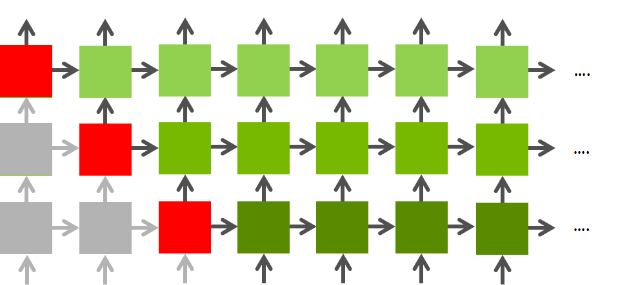
\includegraphics[width=12cm]{wavefront_parallelism.png}
    \caption{Dependency graph for LSTM inference, unrolled over time steps and layers. The horizontal axis corresponds to time steps and the vertical axis corresponds to layers. Gray denotes cells that have already completed execution. Red denotes cells that can be executed in parallelism under layer-wise parallelism. This figure is taken from an NVidia blog post~\cite{nvidia_lstm}.}
    \label{fig:wavefront_parallelism}
\end{figure}

% Explain wavefront parallelism
The main parallelization strategy that we investigate in this project is the previously mentioned layer-wise parallelism, a type of wavefront parallelism.
As illustrated in Figure~\ref{fig:wavefront_parallelism}, the dependency graph of LSTM inference can be unrolled over time to form a 2D grid. The execution of a cell requires the completion of the same layer at the previous time step and the previous layer at the current time step.
In general, wavefront parallelism is suitable for this type of dependency graph, as different columns of multiple rows can be executed simultaneously. For instance, in Figure~\ref{fig:wavefront_parallelism}, given the completion of the gray cells, the red cells can be all executed in parallel.

% Describe central task queue implementation
% TODO: maybe add a figure illustrating this implementation?
\subsection{Central Queue Implementation (CQ)}
There are many ways of implementing layer-wise parallelism.
The first and most basic method that we came up with involves using a central task queue, where each task corresponds to executing the operations in an LSTM cell at a specific layer and time step.
Since every cell has up to two dependencies, we also need to use a data structure to keep track of which cells have been completed.
Whenever a cell finishes execution, each of its two dependent cells is checked. If all dependencies of a dependent cell have been satisfied, it should be added to the task queue.
The parallelization comes from launching many threads, each of which can grab tasks from the queue to execute and queue new tasks when appropriate.

However, a few problems come with this implementation.
First of all, as a shared resource that can be modified, the task queue methods must be atomic in implementation.
Because threads grab tasks from the queue very often, there will be high contention for the queue, which can incur a high synchronization overhead.
Additionally, adding a dependent cell to the task queue requires checking the other dependency and doing so naively can lead to race conditions.
For instance, let's say that cell C has cells A and B as dependencies.
If cell A and cell B finish executing simultaneously and check whether the other is done, both may see that the other is not done yet.
In this scenario, cell C would never be added to the task queue, causing incorrect behavior.
As a result, some form of synchronization would also be needed for the data structure tracking finished dependencies, leading to additional overhead.

The final implementation made use of an atomic integer \verb|progress| array, which kept track of how many time steps had been completed for each layer. This solves the race conditions mentioned above, since the progress values, which can be used to infer which tasks' dependencies have been completed, are incremented and fetched atomically.  The implementation also attempted to use the queue as little as possible. If a thread finds that a new task is available after updating dependencies due to the completion of a previous task, it will take the new task for itself. Only in the situation where a thread finds that both dependent tasks are now available does it push one of them on the queue. All queue methods were made atomic by giving the queue structure a single atomic boolean which when used with Compare and Swap (CAS) could be used as a lock. 

However, queue contention still lead to this implementation not scaling well, so we moved on to implementations with lower contention on critical resources.

% Describe our current parallelization strategy
% TODO: Definitely make a visualization of how this strategy works OR show pseudo code
\subsection{Loop Scan Implementation (LS)}

In this implementation, instead of having threads grabbing tasks from a central queue, which leads to high contention, each thread repeatedly scans over the time steps and identifies available work to do.
We use two arrays: a \verb|busy| array to indicate whether a time step is being worked on and a \verb|progress| array to track how many layers the input at a time step has gone through.
Each thread continuously loops over all time steps and attempts to work on it.
Since only one thread can work on time step \verb|t| at a time, the thread first uses a CAS operation on \verb|busy[t]| to gain exclusive access.
If the CAS fails, then another thread must be currently working on it. In that case the original thread simply moves onto the next time step.
This is different from using a lock on every time step in that we don't stall until the cell becomes ready.
If the thread gains exclusive access, it then checks whether the dependencies have been met by looking at the \verb|progress| of the previous time step.
If the dependencies are satisfied then the cell is executed.
In either case, exclusive access is relinquished at the end.
Inference ends when \verb|progress| is equal to the depth of the network for all time steps.

% Talk about improvements made
% swapping depth/time steps dimensions
This first version of the implementation was suboptimal and we made several improvements on it.
First of all, in most realistic applications of LSTM models, we have $N \ll T$, where $N$ is the depth of the network / number of layers and $T$ is the number of time steps.
Currently, since we are iterating over the time steps to identify available work, a cell which becomes available may have to wait $T$ iterations before it gets identified.
In other words, the threads waste a lot of time iterating over time steps that are not relevant (either already fully completed or not started at all yet).
To remediate this, we simply made the threads iterate over the layers instead of the time steps.
The \verb|progress| and \verb|busy| arrays are changed to track the layers accordingly.
This small modification means that any cell that is ready will only wait up to $N$ iterations before being picked up which is much better since $N \ll T$.
In addition, we started to keep track of the range of layer indices currently being worked on and only iterate over that to avoid useless work.

% Test & Test & Set
Another inefficiency in this implementation is that since we do a CAS operation at every iteration, there can be high contention (e.g. many threads attempt to do a CAS on the same memory address at the same time).
This also increases the coherence traffic because using a CAS operation requires an exclusive state that invalidates the cache lines of all other threads.
We noticed that many of the CAS operations are unnecessary because the layer may not be ready to execute yet.
To address this issue, we inspired ourselves from the ``test and test and set" implementation that we saw in class and added a conditional statement to check whether the layer is free and ready to execute before attempting the CAS.
This largely reduced contention and the amount of unnecessary CAS operations, and resulted in better speed ups.
% Issue: a lock gets released and many threads all try to use CAS to get the lock (contention + coherence traffic)
Even with the improvement, it is possible that, especially at higher thread counts, when a cell becomes ready to execute, many threads pass the first ``test" simultaneously and we still have contention and high coherence traffic at the CAS.

% Stay at same layer for better memory locality
We made one last improvement to this implementation in order to optimize cache performance.
We noticed that, for a single thread, it is more beneficial to do all of the time steps at a layer before moving onto the next.
The reason behind this is that the hidden and memory states are reused within the same layer.
Staying at the same layer would therefore result in better locality of memory access, improving cache performance.
We modified our implementation such that when a thread updates a layer, it will attempt to stay at that layer instead of moving onto the next layer immediately.
This has a larger effect on computation time for smaller thread counts.

% Describe layer-as-task implementation
\subsection{Layer-as-Task Implementation (LaT)}

One issue with CQ was high contention on a critical resource.
Another way of reducing contention is to have coarser-grained tasks.
In this implementation, we treat an entire layer as a task instead of each individual cells.
We use a counter to indicate the index of the next layer to work on, with each thread using a atomic increment and fetch operation on the counter.
We also keep track of a \verb|progress| array just like in CQ so that a thread can monitor the progress of the previous layer and wait for a dependency to finish running if necessary.
This implementation greatly reduces the contention on critical resources since there are only $N$ tasks, as opposed to $NT$ tasks in the CQ implementation.
The time spent on each request is also lower since an atomic increment operation is likely faster than a push/pop operation for a queue.
In addition, a single thread doing all of the computation in one layer means less synchronization overhead within the layer and better cache performance as explained in our LS implementation.

% TODO: Talk about the downside of this method


\subsection{Implementation Details}
% Programming language
The code for this project is written in C++ and available at \url{https://github.com/mochangheng/Parallel_LSTM}.
% CPU matrix operations (Eigen3)
For vector and matrix operations on CPU, such as element-wise arithmetic operations and matrix multiplication, we used the \href{https://eigen.tuxfamily.org}{Eigen 3} library.
% GPU matrix operations (Cublas + CUDA)
For vector and matrix operations on GPU, we used a combination of the cuBLAS library and our own CUDA kernels.
These libraries were chosen mainly because they have an efficient and easy-to-use parallel matrix multiplication algorithm. 
In order to parallelize over layers, we used the \verb|pthreads| library.


\section{Results}

% NOTE: I think it's better to split the different things we do into separate subsections
% First, we compare the speedups of the three implementations on depth = 64, varying the number of cores
% Second, we investigated whether we should dedicate resources to layer-wise parallelism vs. math parallelism. Batch size is set to 16 to increase the amount of available math parallelism
% Third, we investigated layer-wise parallelism on CPU vs. math parallelism on CUDA (and showing the CUDA is good for higher batch sizes)
% Finally, we show that increasing the number of time steps increases the speedup

\subsection{Comparison of the three implementations}
% We collected data on speedup over a variety of factors. This included number of cores, core assignment (cores parallelizing over layers or cores parallelizing math operations), use of CUDA for GPU parallelization, and batch size.
We compared the performance and speedups of our three implementations by measuring the  wall-clock time spent on computation.
The correctness of our implementations was verified by comparing the output to a baseline, sequential implementation.
For all tests, inputs were randomly generated, as computation time wasn't dependent on the values of the inputs.

\begin{figure}
    \centering
    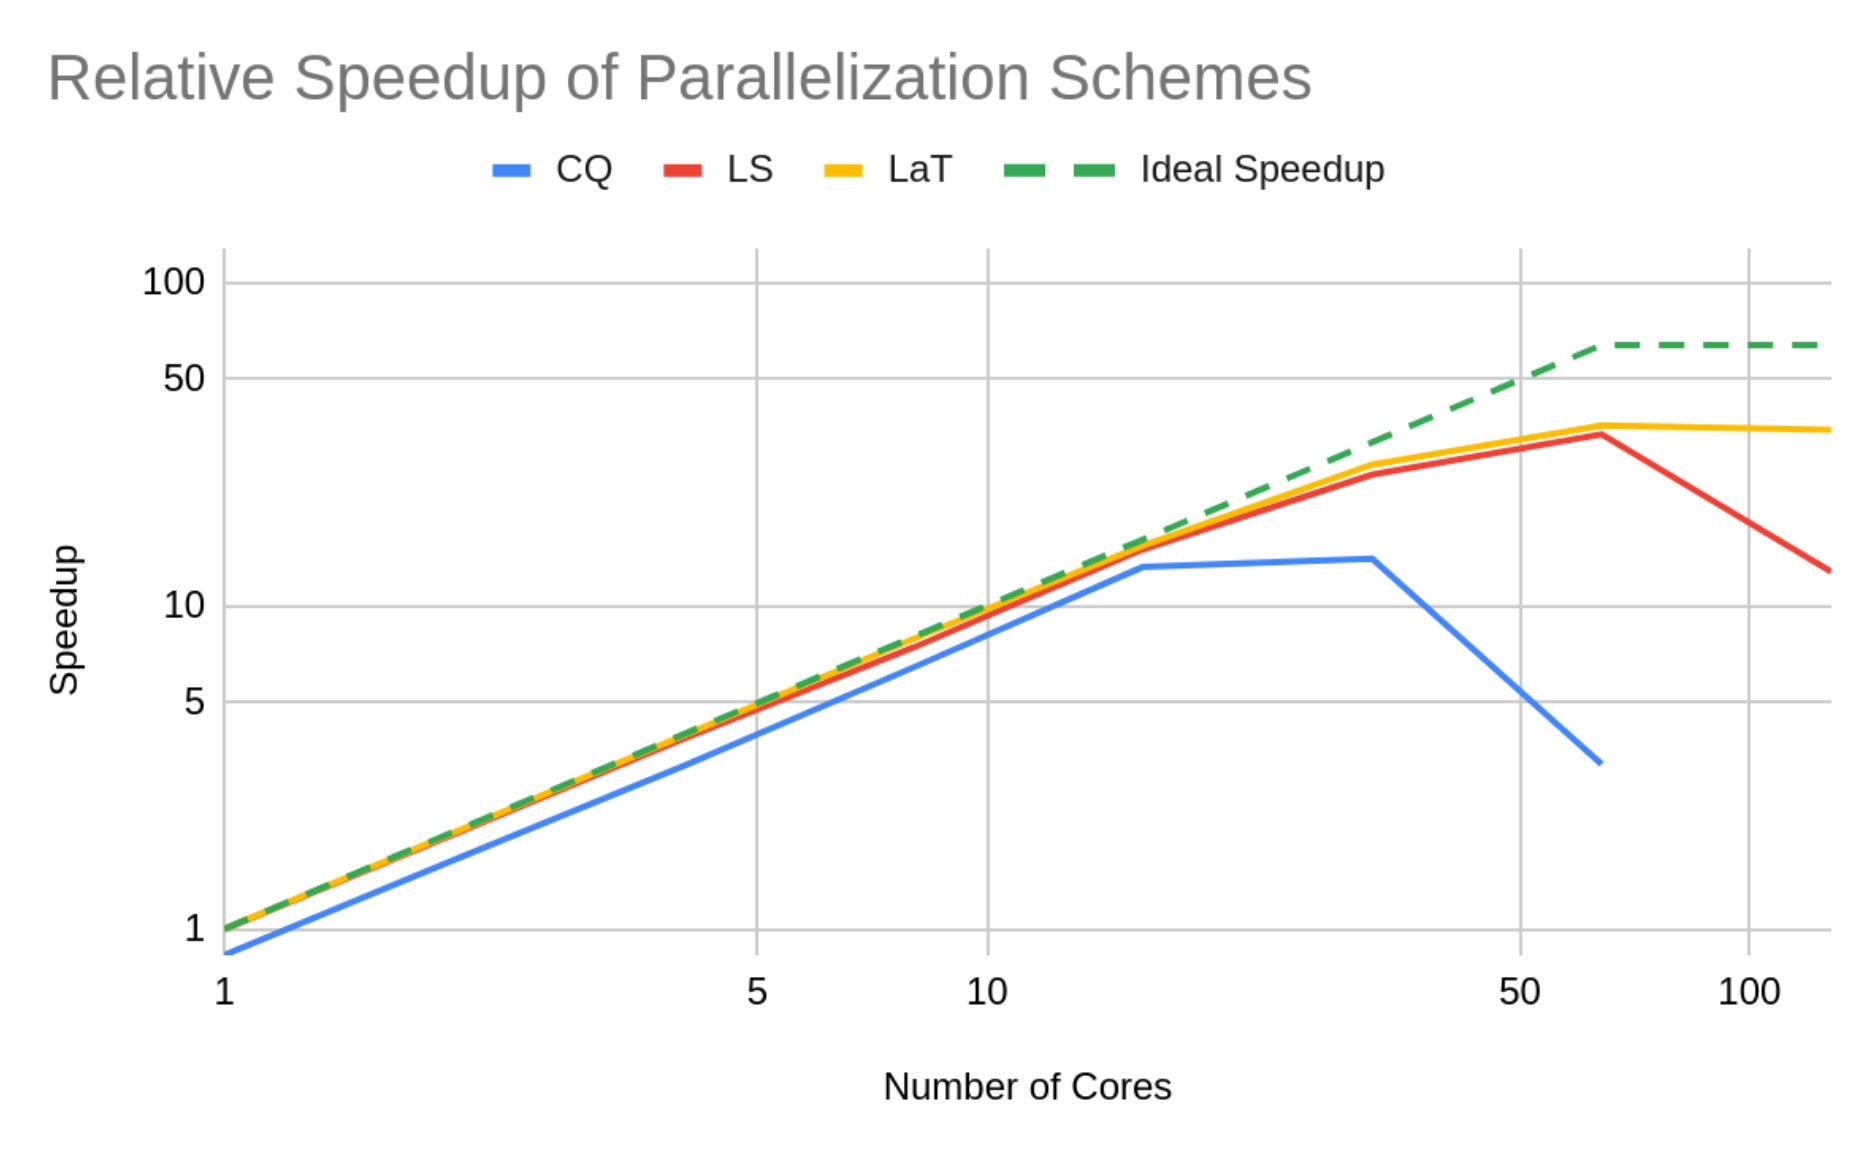
\includegraphics[width=12cm]{speedups.png}
    \caption{The results of running each parallelization scheme on a varying number of cores. Speedup is relative to LaT with one core. $N$ was 64, $T$ was 128, and the size of the hidden vector was 128.}
    \label{fig:scheme_speedups}
\end{figure}

\begin{figure}
    \centering
    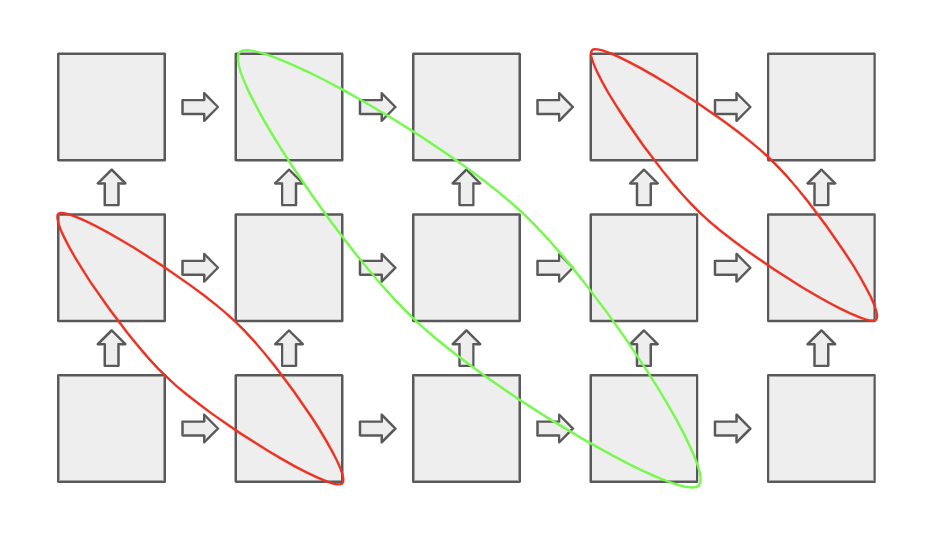
\includegraphics[width=12cm]{dependency.png}
    \caption{An example of how an $N$ = 3, $T$ = 5 LSTM dependency graph has lower widths near the first and last tasks, and a maximum width of $N$ when $N < T$. All squares in a circled group have the same distance from the bottom left starting squre.}
    \label{fig:dependency}
\end{figure}

Figure~\ref{fig:scheme_speedups} shows that the speedup of our parallelization implementations improved iteratively.
As expected, CQ has poorer speedups at higher thread counts due to the issues that we discussed previously.
Both LS and LaT has close to linear speedup up to 32 cores, and sublinear speedup at 64 cores.
Because the depth of the LSTM was 64, it was impossible for 128 cores to be faster than 64 cores. 
We included the 128 core data to see how much additional overhead more cores caused for LS and LaT.
LaT experienced minimal overhead while the speedup of LS degraded significantly.
We didn't test CQ with 128 cores because the speedup has already degraded by a lot at 64 cores.
Overall, LaT has the fastest computation time at each core, proving to be our best implementation.


\subsection{Number of time steps is a bottleneck for parallelism}
We investigated why we don't get perfect speedup and realized that we were constrained by the problem size. The way the dependency graph is structured means that early on there are few tasks to do, much less than there might be cores. Eventually, the width of the dependency graph reaches $\min(N,T)$. Since as stated earlier we assume $N \ll T$, we can simplify this maximum width to our depth $N$. It is at this point we can get the most speedup. However, at the end of the dependency graph it narrows again as we approach the final task, meaning the number of available tasks might again fall below the number of cores (Figure~\ref{fig:dependency}). It is because of the start and end of the dependency graph that perfect speedup cannot be achieved for the computation as a whole. However, this idea would tell us that the skinnier the rectangle of our dependency graph, or mathematically the larger $\frac{T}{N}$ is, the higher the ratio of computation time spent with maximum dependency graph width / parallelizability. This higher ratio would translate to a higher overage speedup overall.
We ran further experiments by increasing the number of time steps in the input.
The results in Figure~\ref{fig:time_steps_versus_speedup} show that, as predicted, we can get more speedup as by increasing $T$.
The remaining reasons why we do not get perfect speedup are speculated to be more general, such as memory bounding issues due to poor math optimizations and synchronization overhead.

\begin{figure}
    \centering
    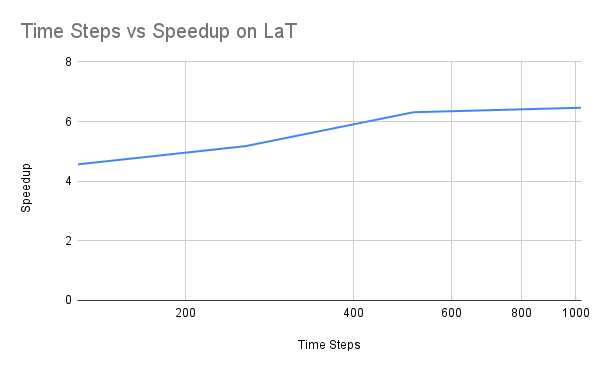
\includegraphics[width=12cm]{Time Steps vs Speedup on LaT.png}
    \caption{The speedups measured were a ratio of computation time for 8 cores over the computation time for 64 cores for varying values of $T$. $N$ was 64 and the size of the hidden vector was 128.}
    \label{fig:time_steps_versus_speedup}
\end{figure}

\subsection{Layer-wise parallelism vs. math parallelism on CPU}
However, all this speedup over layers is no good if these resources can be put to better use elsewhere. As stated in the background, the mathematical operations on matrices in the LSTM cells can be parallelized. As a result, we wanted to see whether it's more efficient to allocate cores to layer-wise parallelism or mathematical parallelism.

\begin{figure}
    \centering
    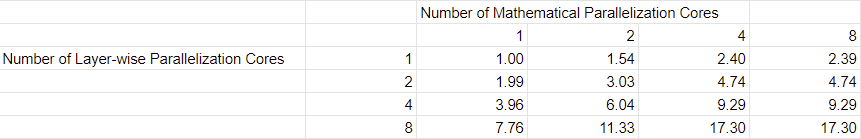
\includegraphics[width=15cm]{table.png}
    \caption{The speedups were measured relative to the computation time with 1 core for both math and layer-wise on LaT. $N$ was 8, $T$ was 128, and the size of the hidden vector was 128. Batch size was set to 16. }
    \label{fig:layerwise_versus_math_cpu}
\end{figure}

We ran a series of tests, varying both the number of cores available for layer-wise and mathematical parallelism using the LaT implementation.
Batch size is defined as the number of simultaneous computations that must be performed.
The batch size was set to 16 in order to increase the amount of mathematical parallelism available.
This means that instead of processing a single input vector, we are processing many of them simultaneously.
Our results, shown in Figure~\ref{fig:layerwise_versus_math_cpu}, show that it is always better to assign resources to layer-wise parallelism over mathematical parallelism. While the best speedup was when both types had resources, situations where they had differing resources always favored more layer-wise cores than math cores.

\begin{figure}
    \centering
    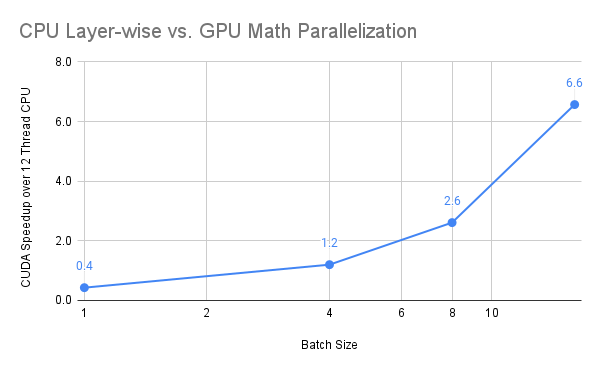
\includegraphics[width=15cm]{CPU Layer-wise vs. GPU Math Parallelization.png}
    \caption{The speedup is the time taken by CPU LaT with 12 threads divided by the time taken by CUDA GPU math parallelization. $N$ was 16, $T$ was 128, and the size of the hidden vector was 128.}
    \label{fig:cpu_versus_gpu}
\end{figure}

\subsection{CUDA parallelism is better for large workloads}
However, those previous results only investigated parallelizing math on the CPU.
Given the nature of the workload, GPU is a better hardware for this kind of parallelization.
This means that in order to grasp the full picture we needed to compare layer-wise parallelization over varying batch sizes to a CUDA version that used the GPU to parallelize the math.

We tested the CPU implementation with 12 cores and the GPU implementations across various batch sizes.
The absolute computation times are not as important.
Figure~\ref{fig:cpu_versus_gpu} found that as batch size increased, the GPU starts to perform much better than the CPU comparatively.
This means that there does exist a situation where focusing on math parallelization is better than focusing on layer-wise. It requires both higher batch size and access to good GPU hardware.

\section{Conclusion}
Overall, our results were positive in that in most situations decent speedup could be achieved through layer-wise parallelism. We were able to settle on a satisfactory implementation that had low overhead due to a lack of shared resources, and only in specific circumstances was this method overshadowed by math parallelism.

\section{Work Distribution}
Owen:
\begin{itemize}
    \item Wrote a baseline, sequential implementation
    \item Wrote the LS and LaT implementations
    \item Wrote the Approach section of the report
    \item Revised the report
    \item Worked on the Background and LS sections of the presentation
\end{itemize}

Jeremy:
\begin{itemize}
    \item Wrote the CQ implementation
    \item Wrote the Summary, Background, Results, Conclusion sections of the report
    \item Revised the report
    \item Worked on the rest of the sections (other than Background and LS sections) of the presentation
\end{itemize}

The work distribution is about 60\% Owen and 40\% Jeremy.

\bibliographystyle{plain}
\bibliography{bibliography}


\end{document}
